\documentclass[preprint]{sigplanconf}

\usepackage[utf8]{inputenc}
% the following standard packages may be helpful, but are not required
\usepackage{longtable}
%\usepackage{mathtools}
\usepackage{multicol}
%\usepackage{multirow}
\usepackage{booktabs}
%\usepackage{courier}
%\usepackage[scaled]{helvet}
\usepackage{url}
\usepackage{listings}
%\usepackage{enumitem}
%\usepackage{mdwlist} % tighter description environment (starred)
%
\usepackage{graphicx}
\usepackage{softdev}
\usepackage{amsmath}
%\usepackage{mdwlist}
%\usepackage{pifont}
\usepackage{xspace}

\newcommand{\kalibera}{Kalibera \& Jones\xspace}
\newcommand{\krun}{Krun\xspace}
\newcommand{\hypone}{H1\xspace}
\newcommand{\hyptwo}{H2\xspace}
\newcommand{\binarytrees}{\emph{binary trees}\xspace}
\newcommand{\richards}{\emph{Richards}\xspace}
\newcommand{\spectralnorm}{\emph{spectralnorm}\xspace}
\newcommand{\nbody}{\emph{n-body}\xspace}
\newcommand{\fasta}{\emph{fasta}\xspace}
\newcommand{\fannkuch}{\emph{fannkuch redux}\xspace}
\newcommand{\bencherthree}{Linux1/i7-4709K\xspace}
\newcommand{\bencherfive}{Linux2/i7-4790\xspace}
\newcommand{\benchersix}{OpenBSD/i7-4790\xspace}
\newcommand{\bencherseven}{ARM\edd{XXX name properly if used}\xspace}

\lstset{
    basicstyle=\tt\scriptsize,
    xleftmargin=2em,
    framexleftmargin=1.5em,
    numberstyle=\scriptsize\tt\color{gray},
    captionpos=b,
    escapeinside={{<!}{!>}},
}

\SDShowCommentTags{default}  %final

\begin{document}

\title{Virtual Machine Warmup Blows Hot and Cold}

\authorinfo{Edd Barrett}
{Software Development Team, Department of Informatics, King's College London}{\texttt{http://eddbarrett.co.uk/}}

\authorinfo{Carl Friedrich Bolz}
{Software Development Team, Department of Informatics, King's College London}{\texttt{http://cfbolz.de/}}

\authorinfo{Rebecca Killick}
{Department of Mathematics and Statistics, University of Lancaster}{\texttt{http://www.lancs.ac.uk/\~{}killick/}}

\authorinfo{Vincent Knight}
{School of Mathematics, Cardiff University}{\texttt{http://vknight.org/}}

\authorinfo{Sarah Mount}
{Software Development Team, Department of Informatics, King's College London}{\texttt{http://snim2.org/}}

\authorinfo{Laurence Tratt}
{Software Development Team, Department of Informatics, King's College London}{\texttt{http://tratt.net/laurie/}}


\maketitle

\section{Introduction}
\label{sec:intro}

Many modern languages are implemented as Virtual Machines (VMs) which use a
Just-In-Time (JIT) compiler to translate `hot' parts of a program into efficient
machine code at run-time. Since it takes time to determine which parts of the
program are hot, and then compile them, programs which are JIT compiled are
said to be subject to a \emph{warmup} phase. The traditional view of
JIT compiled VMs is that program execution is slow during the warmup phase, and
fast afterwards, when \emph{peak performance} is said to have been reached
(see Figure~\ref{fig:trad} for a simplified view of this).
This traditional view underlies most benchmarking of JIT compiled VMs, which
generally aim to measure peak performance.
Typically, benchmarks are run repeatedly in a single process, then data prior
to peak performance is discarded.

The aim of this paper is to test the following hypothesis:
\begin{description}
  \item[\hypone] Small, deterministic programs exhibit traditional warmup behaviour.
\end{description}
In order to test this hypothesis, we present a carefully designed
experiment where a number of simple benchmarks are run on a variety of
VMs for a large number of \emph{in-process iterations} and repeated using fresh
\emph{process executions} (i.e.~each process execution runs multiple in-process
iterations). We deliberately treat VMs as black boxes: we simply run benchmarks
and record timing data.

\begin{figure}[t]
\centering
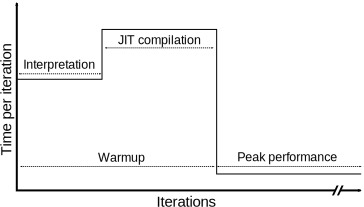
\includegraphics[width=.5\textwidth]{img/picturebook_warmup}
\caption{The traditional notion of warmup: a program starts slowly executing in
an interpreter; once hot parts of the program are identified, they are
translated by the JIT compiler to machine code; at this point warmup
is said to have completed, and peak performance reached.}
\label{fig:trad}
\end{figure}

While some benchmarks on some VMs run as per
traditional expectations, we found a number of surprising cases. At
the most extreme, some benchmarks never warm up, staying at their initial performance
levels indefinitely and some even slowdown. Of the eight
VMs we looked at, none consistently warmed under the traditional model.

Our results clearly invalidate H1: the traditional view of warmup is no longer
valid. We are not aware that anyone has systematically noted this
problem before, let alone take it into account when benchmarking. This suggests
that many published VM benchmarks (including our own) may have presented
results which are misleading in some situations.

We believe that accurate VM benchmarking is paramount, for both VM authors, and
for many end users. VM authors need to know if optimisations have an effect
distinguishable from noise (and many optimisations have only a small effect).
Similarly, end-users with latency sensitive workloads (e.g. games or other soft
real-time systems) rely upon accurate benchmarking during their evaluation
phase. Our results suggest that current benchmarking methodology is leading
these parties astray.

\section{Background}
\label{sec:warmup}

When a program begins running on a JIT compiled VM, it is typically (slowly)
interpreted; once `hot' (i.e.~frequently executed) loops or methods are
identified, they are compiled into machine code; and subsequent
executions of those loops or methods use (fast) machine code rather than the
(slow) interpreter. Once machine code generation has completed, the VM is
traditionally said to have finished warming up, and the program to be executing
at peak performance.\footnote{This traditional notion applies equally to VMs
that perform immediate compilation instead of using an interpreter, and to
those VMs which have more than one layer of JIT compilation (later JIT
compilation is used for `very hot' portions of a program, and tolerates slower
compilation time for better machine code generation).}

Figure~\ref{fig:trad} illustrates a
program subject to the conventional model of warmup. Exactly how long warmup
takes is highly dependent on
the program and the JIT compiler, but this basic assumption about the
performance model is shared by every JIT compiling
VM~\cite{kalibera13rigorous}.

Benchmarking of JIT compiled VMs typically focusses on peak
performance. in large part because the widespread assumption has been that
warmup is both fast and inconsequential to users. With that assumption in mind, the
methodologies used are typically straightforward: benchmarks are run for a number
of in-process iterations within a single VM process execution.
The first $n$ in-process iterations are then discarded, on the basis that warmup
will have completed at some point before $n$. It is common for
$n$ to be a hard-coded number, e.g. 5. The more sophisticated \kalibera
benchmarking methodology~\cite{kalibera12quantifying,kalibera13rigorous}
(recently used in~\cite{barrett15approaches,grimmer15dynamically}) improves
upon this by having the user manually inspect run-sequence plots (or trace
plots) for each process execution. The method also suggests a method for
dealing with benchmarks which are cyclic in nature (e.g. that produce a
saw-tooth wave when plotted).

While the \kalibera methodology is certainly an improvement over
straightforward benchmarking methodologies,
our experience has been that there remain cases where it is hard to produce
satisfying benchmarking statistics. Crucially, the methodology does not
provide a firm way of determining when warmup has completed. Because of this
``determining when a system has warmed up, or even providing a
rigorous definition of the term, is an open research problem''~\cite{seaton15phd}.

\section{Methodology}
\label{sec:methodology}

To test Hypothesis \hypone, we designed an experiment which uses a suite of
micro-benchmarks: each is run with 2000 in-process iterations and repeated
using 10 process executions. So as
to collect high-quality data, we have carefully designed our
experiment to be repeatable and to control as many potentially confounding variables as
is practical.

The micro-benchmarks we use are as follows: \binarytrees, \spectralnorm, \nbody,
\fasta, and \fannkuch from the Computer Language Benchmarks Game (CLBG); and
\richards. Readers can be forgiven for initial scepticism about this set of micro-benchmarks.
They are small and widely
used by VM authors as optimisation targets.
In our context, this weakness is in fact a strength: we need
small, deterministic, and widely examined programs so that we can test
Hypothesis \hypone. If we were to find unusual warmup behaviours from arbitrary programs,
VM authors might reasonably counter that
``you have found the one program that exhibits unusual warmup behaviour''.

We used C, Java, Javascript, Python, Lua, PHP,
and Ruby versions of each benchmark.\footnote{Our need to have implementations in a wide variety
of languages restricted the micro-benchmarks we could use.} Since most of these
benchmarks have multiple implementations in any given language, we picked
the same versions used in~\cite{bolz14impact}, which represented the fastest
performers at the point of that publication. We were forced to skip some
benchmark and VM pairings which either ran prohibitively slowly
(Fasta/JRubyTruffle and Richards/HHVM), or caused the VM to crash
(SpectralNorm/JRubyTruffle). The benchmarks were audited for ``CFG
determinism'', meaning that no two in-process iterations take different paths
through the control flow graph of the benchmark. We also checked that the
different language versions of the benchmarks all computed the same result.
For the avoidance of doubt we did not interfere with any VM's Garbage
Collection (GC) (e.g.~we did not force a collection after each iteration).

Our benchmarking hardware consisted of three machines:

\begin{description}
\item[\bencherthree] Quad-core i7-4790K 4GHz, 24GB of RAM, running Debian 8.
\item[\bencherfive] Quad-core i7-4790 3.6GHz, 32GB of RAM, running Debian 8.
\item[\benchersix] Identical hardware to \bencherfive, but running OpenBSD 5.8.
\end{description}

\noindent We disabled any hardware features (where possible) that could
possibly induce variation into our results. For example turbo boost and
hyper-threading were disabled.

The benchmarks were then run on the following VMs: GCC 4.9.3; Graal 0.13;
HHVM 3.12.0; a recent GIT version of JRuby/Truffle\footnote{GIT
hash: \texttt{f82ac77137da265d2447d723ce5973a04459a609}}; HotSpot 8u72b15;
LuaJIT 2.0.4; PyPy 4.0.1; and V8 4.9.385.21. Although not a VM, GCC serves as a
baseline to compare the VMs against. HHVM and JRuby/Truffle do not yet run on
OpenBSD, and were thus skipped on the OpenBSD benchmarking machine.
We use a script to downloads, configures, and build the above
versions of the VMs, ensuring we can easily repeat builds. All VMs were
compiled with a manually built GCC/G++ 4.9.3 (the same used for C benchmarks),
thus eliminating the GCC versions themselves as a source of variation.

The benchmarks were run under a specially developed tool called \krun, which
measures in-process iteration times (using a monotonic clock) whilst in a
fashion which minimises the effect of external sources of variation. To name a
few features, \krun: reboots the system prior to the first process execution
and after each process execution; ensures that each process execution starts
with the same system temperatures; runs benchmarks as an otherwise unused user
account; and (on Linux, where this is possible) runs the kernel with
adaptive-tick mode CPU cores~\cite{tickless}.

\section{Preliminary Results}
\label{sec:Results}

Our experiment runs 450 unique process executions, giving a total of 900\,000
in-process iteration readings. For each process execution we generate a
run-sequence graph, with the in-process iteration number on the $x$ axis, and the
time (in seconds) on the $y$ axis. A full set of graphs, as well as our raw
data, can be downloaded from:
\vspace{-1em}
\begin{center}
{\small%
\url{https://archive.org/download/softdev_warmup_experiment_artefacts/v0.2/}
}
\end{center}

Although some of the graphs do show classical warmup behaviour
(Figures~\ref{fig:good1,fig:good2}, others highlight a number of interesting
features:

\begin{description}
%\item[Outliers] In-process iterations which are slower (or, less commonly, much
%faster) than neighbouring in-process iterations. E.g. Figure~\ref{fig:outliers}.
\item[Cycles] In-process iteration times repeat in a predictable pattern. E.g.
Figure~\ref{fig:cycles}.
\item[Slowdown] Performance of in-process iterations drops over time. E.g.
Figure~\ref{fig:slowdown}.
\item[Changing phases] The mean of in-process iteration times abruptly changes
over time. E.g. Figure~\ref{fig:phases}.
\item[Inconsistent process executions] Process executions for the same
benchmark / VM pair behave differently. Sometimes this occurs on in-process
executions on the same machine; sometimes only across machines. E.g.
Figure~\ref{fig:inconsistent}.
\end{description}

The preliminary results are troubling. Process executions which do not warmup
under the classical model cannot have traditional benchmarking methodologies
applied. In other words, if the end of the warmup phase cannot be identified,
then in turn the peak performance phase cannot be identified. This suggests
that benchmarking methodologies need to be rethought.


\section{Related work}

There are two works we are aware of which explicitly note unusual warmup
patterns. Gil et al.'s main focus is on non-determinism of process executions on
HotSpot, and the difficulties this raises in terms of providing reliable
benchmarking numbers~\cite{gil11microbenchmark}. The authors report
process executions which we would classify as a slowdowns. \kalibera note the
existence of what we have called cyclic behaviour (in the context of benchmarking,
they then require the user to
manually pick one part of the cycle for measurement~\cite{kalibera13rigorous}).

\section{Conclusions and Future Work}
\label{sec:conclusion}

Warmup has always been an informally defined term~\cite{seaton15phd} this
preliminary work has shown cases where the definition fails to hold.
To the best of our knowledge, we are the first to (informally) classify different
`warmup' styles and note the relatively high frequency of non-traditional
classifications such as slowdown and phase changes.
However, we have not yet found an acceptable alternative definition of warmup.
Based on our experiences thus far, we think it unlikely that the different
styles of warmup we have seen can be captured in a single metric. We suspect it
is more likely that a number of different metrics will be needed to describe and
compare warmup styles.

There are several items of potential future work which would likely lead to a
better understanding of the warmup behaviours: automated classification of
warmup behaviours would help guide us through the vast amount of data we have
collected.\footnote{We have already started this task.}; VM instrumentation may
help us pair VM events (compilation, GC, \ldots). Similarly we should look at
hardware performance counters in-case steps and spikes are due to hardware
events (context switches, CPU migrations, \ldots).

\textbf{Acknowledgements:} This research was funded by the EPSRC Cooler
(EP/K01790X/1) grant and Lecture (EP/L02344X/1) fellowship.

\bibliographystyle{plainnat}
\bibliography{bib}


\begin{figure*}[ch]
%\makebox[\textwidth][c]{
\includegraphics[width=\textwidth]{examples_v2_results/bad_inconsistent.pdf}
%}
\caption{Inconsistent process executions on the same machine.}
\label{fig:inconsistent}
\end{figure*}

\begin{figure}[ch]
\includegraphics[width=.5\textwidth]{examples_v2_results/good_fast.pdf}
\caption{A process execution showing fast classical warmup.}
\label{fig:good1}
\end{figure}

\begin{figure}[ch]
\includegraphics[width=.5\textwidth]{examples_v2_results/good_tiers.pdf}
\caption{A process execution showing (long, but) classical warmup.}
\label{fig:good2}
\end{figure}

% Not sure if I want this yet.
%\begin{figure}[c]
%\includegraphics[width=.5\textwidth]{examples_v2_results/good_gc.pdf}
%\caption{A process execution with outliers.}
%\label{fig:outliers}
%\end{figure}

\begin{figure}[ch]
\includegraphics[width=.5\textwidth]{examples_v2_results/bad_cycles.pdf}
\caption{A process execution with cycles.}
\label{fig:cycles}
\end{figure}


\begin{figure}[ch]
\includegraphics[width=.5\textwidth]{examples_v2_results/bad_slowdown.pdf}
\caption{A process execution with slowdown.}
\label{fig:slowdown}
\end{figure}

\begin{figure}[ch]
\includegraphics[width=.5\textwidth]{examples_v2_results/bad_phases.pdf}
\caption{A process execution with changing phases.}
\label{fig:phases}
\end{figure}

\end{document}

